%%%%%%%%%%%%%%%%%%%%%%%%%%%%%%%%%%%%%%%%%
% University Assignment Title Page 
% LaTeX Template
% Version 1.0 (27/12/12)
%
% This template has been downloaded from:
% http://www.LaTeXTemplates.com
%
% Original author:
% WikiBooks (http://en.wikibooks.org/wiki/LaTeX/Title_Creation)
%
% License:
% CC BY-NC-SA 3.0 (http://creativecommons.org/licenses/by-nc-sa/3.0/)
% 
% Instructions for using this template:
% This title page is capable of being compiled as is. This is not useful for 
% including it in another document. To do this, you have two options: 
%
% 1) Copy/paste everything between \begin{document} and \end{document} 
% starting at \begin{titlepage} and paste this into another LaTeX file where you 
% want your title page.
% OR
% 2) Remove everything outside the \begin{titlepage} and \end{titlepage} and 
% move this file to the same directory as the LaTeX file you wish to add it to. 
% Then add \input{./title_page_1.tex} to your LaTeX file where you want your
% title page.
%
%%%%%%%%%%%%%%%%%%%%%%%%%%%%%%%%%%%%%%%%%
%\title{Title page with logo}
%----------------------------------------------------------------------------------------
%	PACKAGES AND OTHER DOCUMENT CONFIGURATIONS
%----------------------------------------------------------------------------------------

\documentclass[12pt]{article}
\usepackage[english]{babel}
\usepackage[utf8x]{inputenc}
\usepackage{amsmath}
\usepackage{graphicx}
\usepackage[colorinlistoftodos]{todonotes}
\usepackage{listings}
\usepackage[hmargin=2cm]{geometry}

\usepackage{color}
 
\definecolor{codegreen}{rgb}{0,0.6,0}
\definecolor{codegray}{rgb}{0.5,0.5,0.5}
\definecolor{codepurple}{rgb}{0.58,0,0.82}
\definecolor{backcolour}{rgb}{0.95,0.95,0.92}
 
\lstdefinestyle{mystyle}{
    backgroundcolor=\color{backcolour},   
    commentstyle=\color{codegreen},
    keywordstyle=\color{magenta},
    numberstyle=\tiny\color{codegray},
    stringstyle=\color{codepurple},
    basicstyle=\footnotesize,
    breakatwhitespace=false,         
    breaklines=true,                 
    captionpos=b,                    
    keepspaces=true,                 
    numbers=left,                    
    numbersep=5pt,                  
    showspaces=false,                
    showstringspaces=false,
    showtabs=false,                  
    tabsize=2
}
 
\lstset{style=mystyle}


\begin{document}

\begin{titlepage}

\newcommand{\HRule}{\rule{\linewidth}{0.5mm}} % Defines a new command for the horizontal lines, change thickness here

\center % Center everything on the page
 
%----------------------------------------------------------------------------------------
%	HEADING SECTIONS
%----------------------------------------------------------------------------------------

\textsc{\LARGE Universidad de Granada}\\[1.5cm] % Name of your university/college
\textsc{\Large Algorítmica}\\[0.5cm] % Major heading such as course name
\textsc{\large Memoria de Prácticas}\\[0.5cm] % Minor heading such as course title

%----------------------------------------------------------------------------------------
%	TITLE SECTION
%----------------------------------------------------------------------------------------

\HRule \\[0.4cm]
{ \huge \bfseries Práctica I: Eficiencia}\\[0.4cm] % Title of your document
\HRule \\[1.5cm]
 
%----------------------------------------------------------------------------------------
%	AUTHOR SECTION
%----------------------------------------------------------------------------------------

\begin{minipage}{0.4\textwidth}
\begin{flushleft} \large
\emph{Autora:}\\
Elena Merelo Molina \textsc{} % Your name
\end{flushleft}
\end{minipage}
~
\begin{minipage}{0.4\textwidth}
\begin{flushright} \large
\emph{} \\
\textsc{} % Supervisor's Name
\end{flushright}
\end{minipage}\\[2cm]

% If you don't want a supervisor, uncomment the two lines below and remove the section above
%\Large \emph{Author:}\\
%John \textsc{Smith}\\[3cm] % Your name

%----------------------------------------------------------------------------------------
%	DATE SECTION
%----------------------------------------------------------------------------------------

{\large 13 de Marzo}\\[2cm] % Date, change the \today to a set date if you want to be precise

%----------------------------------------------------------------------------------------
%	LOGO SECTION
%----------------------------------------------------------------------------------------


\includegraphics{logo.png}\\[1cm] % Include a department/university logo - this will require the graphicx package
 
%----------------------------------------------------------------------------------------

\vfill % Fill the rest of the page with whitespace

\end{titlepage}

%\todo[inline, color=green!40]{This is an inline comment.}
%\todo{Here's a comment in the margin!}
% Commands to include a figure:
%\begin{figure}
%\centering
%\includegraphics[width=0.5\textwidth]{frog.jpg}
%\caption{\label{fig:frog}This is a figure caption.}
%\end{figure}


%\section{Análisis de la Eficiencia}


\subsection{Algoritmo de Inserción}
\begin{lstlisting}[language=C]
inline static void insercion(int T[], int num_elem)
{
  insercion_lims(T, 0, num_elem);
}

static void insercion_lims(int T[], int inicial, int final)
{
  int i, j;
  int aux;
  for (i = inicial + 1; i < final; i++) {
    j = i;
    while ((T[j] < T[j-1]) && (j > 0)) {
      aux = T[j];
      T[j] = T[j-1];
      T[j-1] = aux;
      j--;
    };
  };
}
\end{lstlisting}

Vamos a estudiar el peor caso que se le podría presentar al algoritmo de inserción, es decir, que el vector estuviera ordenado en orden inverso (de mayor a menor).

Como vemos en la línea 5, siempre se llama al método con los argumentos $0$ y $num\_elem$, por lo que a partir de ahora para nosotros, $inicial$ será $0$ y $final$ será $n$.

La mayor parte del tiempo de ejecución se emplea en el cuerpo del bucle $while$ interno. Ese trozo de código se puede acotar por una constante $a$. Por lo tanto, las líneas 15-19 se ejecutan un número de veces dependiente del bucle externo, exactamente $i$ veces (ya que estamos suponiendo que nos encontramos en el peor caso). El bucle externo se ejecuta exactamente $n$ veces, por lo que nos queda:

\[T(n)=\sum_{i=1}^{n-1}\sum_{j=1}^{i}a=a\sum_{i=0}^{n-1}\sum_{j=1}^{i}1=a\sum_{i=0}^{n-1}i=a\frac{n(n-1)}{2}\]
Por lo que vemos que $T(n)\in O(n^2)$ o cuadrático.

\subsection{Algoritmo QuickSort}
\begin{lstlisting}[language=C]

static void heapsort(int T[], int num_elem)
{
  int i;
  for (i = num_elem/2; i >= 0; i--)
    reajustar(T, num_elem, i);
  for (i = num_elem - 1; i >= 1; i--)
    {
      int aux = T[0];
      T[0] = T[i];
      T[i] = aux;
      reajustar(T, i, 0);
    }
} 

static void reajustar(int T[], int num_elem, int k)
{
  int j;
  int v;
  v = T[k];
  bool esAPO = false;
  while ((k < num_elem/2) && !esAPO)
    {
      j = k + k + 1;

      if ((j < (num_elem - 1)) && (T[j] < T[j+1])) j++;
      if (v >= T[j]) esAPO = true;
      
      T[k] = T[j];
      k = j;
    }
  T[k] = v;
}
\end{lstlisting}

Vemos que en el primer bucle de la función $heapsort$ aparece la función $reajustar$, por lo que vamos a calcular su eficiencia primero. 

Vemos que el cuerpo del bucle $while$ consume la mayor parte del tiempo de ejecución. El cuerpo de bucle se puede acotar por una constante $b$. Como vemos en la línea 22, el bucle empieza en $k$ y termina en $\frac{n}{2}$, pero $k$ no avanza de 1 en 1, sino de $2k+1$ en $2k+1$, por lo que como mucho se ejecutará $\log(n/2)$ veces. Por lo que $R(n) \in O(\log(n))$, siendo $K(n)$ la función de eficiencia de la función $reajustar$.
Una vez conocida la eficiencia de la función $reajustar$, pasamos a estudiar el primer bucle de la función $heapsort$. Va desde $n/2$ hasta $0$, así que se ejecuta $n/2$ veces, y en cada una de esas veces ejecuta la función $reajustar$, por lo que encontes su eficiencia es $\frac{nlog(n)}{2}$. El segundo bucle se ejecuta $n-1$ veces, por lo que nos queda:
\[T(n)=\frac{nlog(n)}{2}+(n-1)\]
Por lo que $T(n)\in O(n\log(n))$.

\subsection{Algoritmo de Floyd}
\begin{lstlisting}[language=C]
void Floyd(int **M, int dim)
{
	for (int k = 0; k < dim; k++)
	  for (int i = 0; i < dim;i++)
	    for (int j = 0; j < dim;j++)
	      {
				int sum = M[i][k] + M[k][j];    	
		    M[i][j] = (M[i][j] > sum) ? sum : M[i][j];
	      }
}
\end{lstlisting}

Vemos que el cuerpo del tercer bucle $while$ anidado consume la mayor parte del tiempo de ejecución, por lo que lo acotamos por una constante $a$. Fácilmente vemos que el resto de bucles va desde 0 hasta $dim$, que podemos denominar $n$ para mayor facilidad. Por lo que evidentemente tenemos que la eficiencia de este algoritmo es $an^3$, es decir, $T(n)\in O(n^3)$.

%\begin{minipage}{.5\textwidth}
%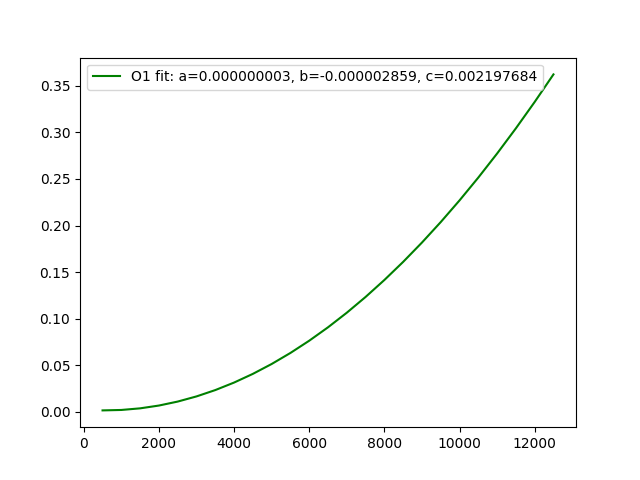
\includegraphics[scale=0.4]{../graficos/burbuja/burbuja_O1.png}  
%\end{minipage}

%\section{Eficiencia Empírica}

%Escribir aqui explicacion del script.

\section{Eficiencia empírica}

En esta práctica veremos la eficiencia empírica de los algoritmos:

\begin{center}
\begin{tabular}{| c | c |}
\hline
Algoritmo & Orden de Eficiencia \\ \hline
Burbuja & O$(n^2$) \\ \hline
Inserción & O$(n^2$) \\ \hline 
Selección & O$(n^2$) \\ \hline 
Mergesort & O$(n\log(n)$) \\ \hline 
Quicksort & O$(n\log(n)$) \\ \hline 
Heapsort & O$(n\log(n)$) \\ \hline
Floyd & O$(n^3)$ \\ \hline 
Hanoi & O$(2^n)$ \\ \hline 
\hline
\end{tabular}
\end{center}
Con el objetivo de estudiar la eficiencia empírica de los algoritmos dados, en cada programa hemos medido el tiempo que ha tardado en ejecutarse, incluyendo la biblioteca ctime y usando clock\_t, compilando cada programa por separado con g++ nombre\_algoritmo.cpp -o nombre\_algoritmo, esto mismo con la opción -O1 y -O3 para luego comparar resultados. 
Cuando ya se generaron los ejecutables, creados para veinticinco valores diferentes de $n$, programa por programa, de manera que los resultados se guarden en sus correspondientes archivos .csv, lo hemos representado ajustando por el método de los mínimos cuadráticos según el orden de eficiencia de cada uno:
\begin{enumerate}
\item $O(n^2)$ ajustada a $f(x)=ax^2+bx+c$
\item $O(n\log(n)$ ajustada a $f(x)=a\log(bn)+c$
\item $O(n^3)$ ajustada a $f(x)=ax^3+bx^2+cx+d$
\item $O(2^n)$ ajustada a $f(x)=a2^{bn}+c$
\end{enumerate}

Vemos ahora detalladamente la representación gráfica de los datos obtenidos.


\newpage
\subsection{Algoritmo burbuja}
\begin{center}
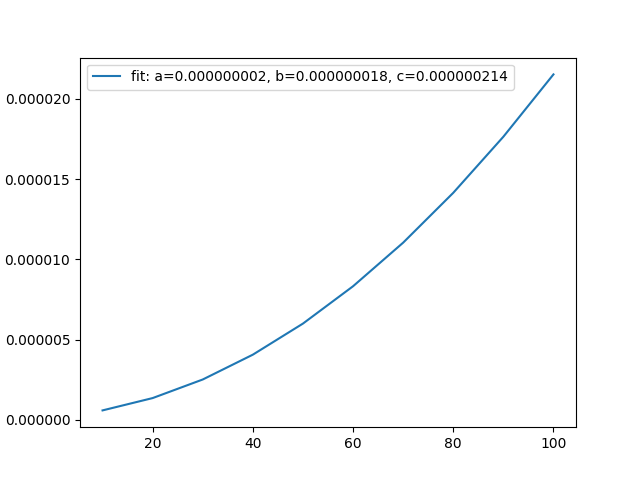
\includegraphics[width=.4\textwidth]{../graficos/burbuja/burbuja.png}
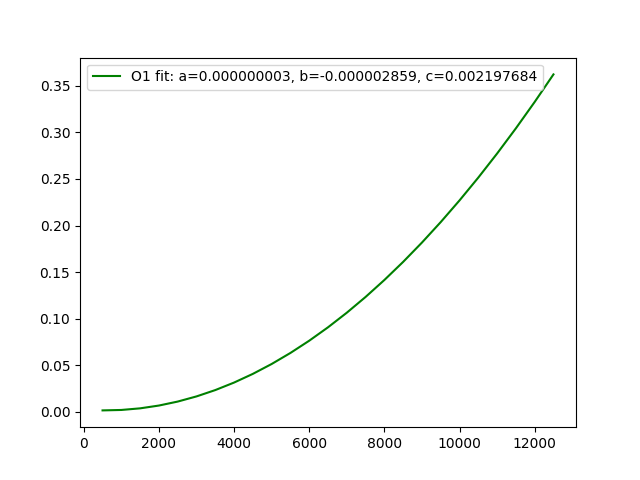
\includegraphics[width=.4\textwidth]{../graficos/burbuja/burbuja_O1.png}
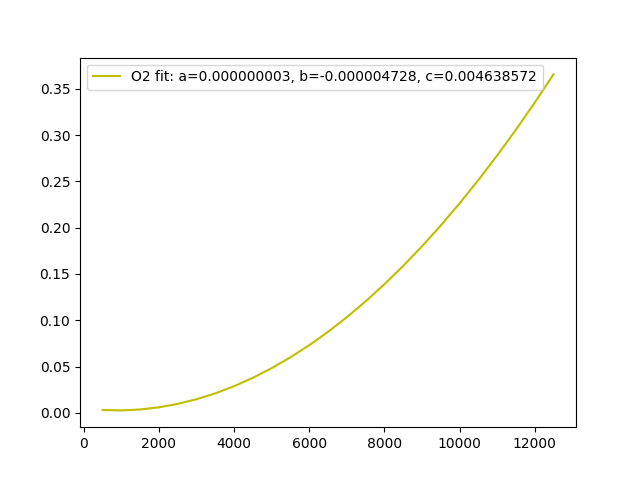
\includegraphics[width=.4\textwidth]{../graficos/burbuja/burbuja_O2.png}
\end{center}
\begin{center}
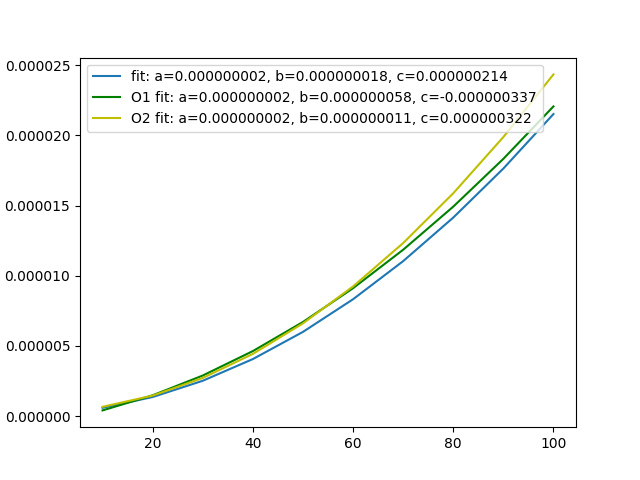
\includegraphics[width=.6\textwidth]{../graficos/burbuja/burbuja_juntas.png}
\end{center}
\begin{center}
\begin{tabular}{| c | c | c | c |}
\hline
\textbf{N} & \textbf{O-} & \textbf{O1} & \textbf{O2} \\ \hline
500 & 0.000848284 & 0.000504565 & 0.000444922 \\ \hline
1000 & 0.00155837 & 0.00170106 & 0.00172926 \\ \hline
1500 & 0.00375233 & 0.00372675 & 0.00348126 \\ \hline
2000 & 0.00625636 & 0.00654731 & 0.00675332 \\ \hline
2500 & 0.0102962 & 0.0111093 & 0.00993443 \\ \hline
3000 & 0.0158037 & 0.0156202 & 0.0159983 \\ \hline
3500 & 0.0211397 & 0.0220235 & 0.021973 \\ \hline
4000 & 0.0292756 & 0.0298859 & 0.0299241 \\ \hline
4500 & 0.0377767 & 0.0425379 & 0.0370894 \\ \hline
5000 & 0.0472146 & 0.0575588 & 0.0466534 \\ \hline
5500 & 0.0585254 & 0.0650413 & 0.0596688 \\ \hline
6000 & 0.0734717 & 0.0795291 & 0.0789712 \\ \hline
6500 & 0.0875871 & 0.0864143 & 0.0938704 \\ \hline
7000 & 0.101356 & 0.106416 & 0.10351 \\ \hline
7500 & 0.119825 & 0.117833 & 0.118222 \\ \hline
8000 & 0.13685 & 0.142887 & 0.13587 \\ \hline
8500 & 0.158619 & 0.156353 & 0.154324 \\ \hline
9000 & 0.177794 & 0.180205 & 0.179462 \\ \hline
9500 & 0.199033 & 0.208484 & 0.197654 \\ \hline
10000 & 0.225543 & 0.224484 & 0.224071 \\ \hline
10500 & 0.249815 & 0.252788 & 0.247328 \\ \hline
11000 & 0.279319 & 0.277287 & 0.284709 \\ \hline
11500 & 0.30519 & 0.305155 & 0.305884 \\ \hline
12000 & 0.335826 & 0.334685 & 0.339147 \\ \hline
12500 & 0.368191 & 0.361129 & 0.365015 \\ \hline
\hline
\end{tabular}
\end{center}
\newpage
\subsection{Algoritmo insercion}
\begin{center}
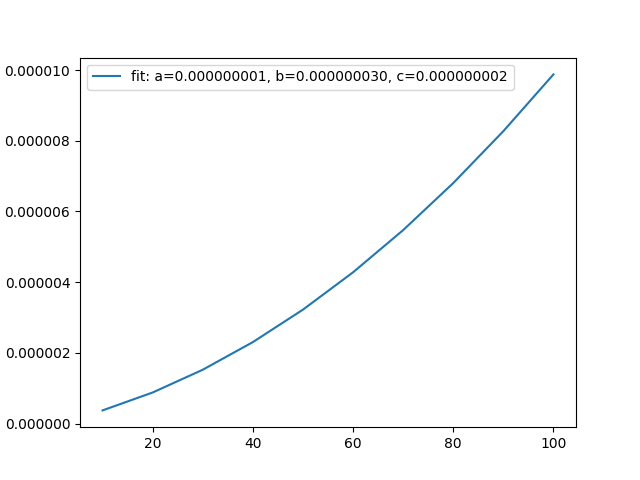
\includegraphics[width=.4\textwidth]{../graficos/insercion/insercion.png}
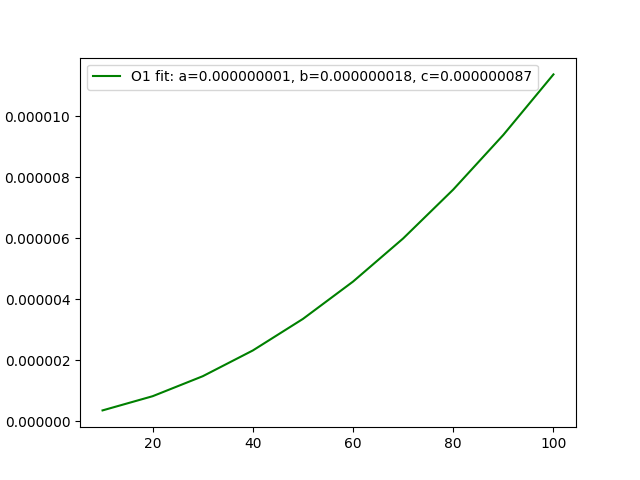
\includegraphics[width=.4\textwidth]{../graficos/insercion/insercion_O1.png}
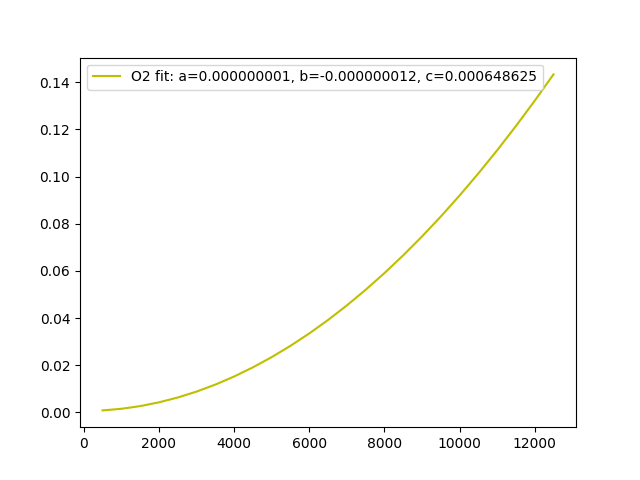
\includegraphics[width=.4\textwidth]{../graficos/insercion/insercion_O2.png}
\end{center}
\begin{center}
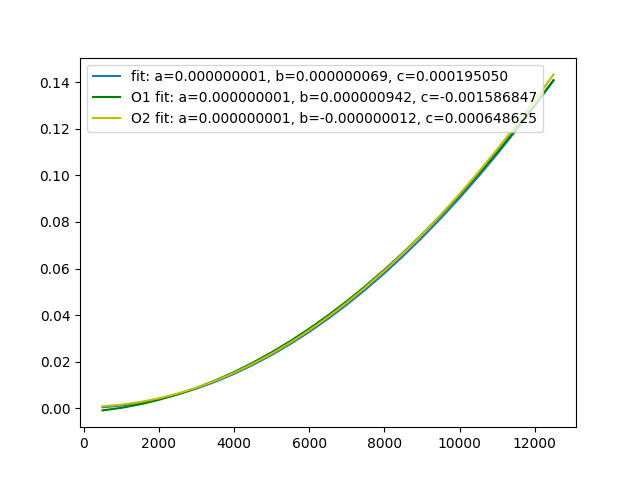
\includegraphics[width=.6\textwidth]{../graficos/insercion/insercion_juntas.png}
\end{center}
\begin{center}
\begin{tabular}{| c | c | c | c |}
\hline
\textbf{N} & \textbf{O-} & \textbf{O1} & \textbf{O2} \\ \hline
500 & 0.000280816 & 0.000233787 & 0.000223985 \\ \hline
1000 & 0.000985635 & 0.000910265 & 0.00100876 \\ \hline
1500 & 0.00213929 & 0.00200899 & 0.00204243 \\ \hline
2000 & 0.00369846 & 0.00377572 & 0.00449 \\ \hline
2500 & 0.00592036 & 0.00560895 & 0.00585753 \\ \hline
3000 & 0.00822953 & 0.00840262 & 0.00825681 \\ \hline
3500 & 0.0120226 & 0.0115001 & 0.0129874 \\ \hline
4000 & 0.0148672 & 0.0151695 & 0.0168938 \\ \hline
4500 & 0.0193506 & 0.0185337 & 0.0193503 \\ \hline
5000 & 0.0227202 & 0.0235869 & 0.0230816 \\ \hline
5500 & 0.0272918 & 0.0275996 & 0.0280322 \\ \hline
6000 & 0.0333669 & 0.0314578 & 0.0388916 \\ \hline
6500 & 0.0395249 & 0.0369619 & 0.0393369 \\ \hline
7000 & 0.0438121 & 0.0443715 & 0.0442169 \\ \hline
7500 & 0.0510923 & 0.0534808 & 0.0519345 \\ \hline
8000 & 0.0577335 & 0.0668524 & 0.0582985 \\ \hline
8500 & 0.0664888 & 0.0740554 & 0.0659169 \\ \hline
9000 & 0.0721457 & 0.0740537 & 0.0733521 \\ \hline
9500 & 0.0804506 & 0.0808475 & 0.081258 \\ \hline
10000 & 0.0889614 & 0.089042 & 0.0897421 \\ \hline
10500 & 0.098722 & 0.0999622 & 0.0988874 \\ \hline
11000 & 0.10898 & 0.111618 & 0.108517 \\ \hline
11500 & 0.120852 & 0.118909 & 0.125629 \\ \hline
12000 & 0.129697 & 0.128718 & 0.137064 \\ \hline
12500 & 0.141071 & 0.140754 & 0.141494 \\ \hline
\hline
\end{tabular}
\end{center}

\newpage
\subsection{Algoritmo seleccion}
\begin{center}
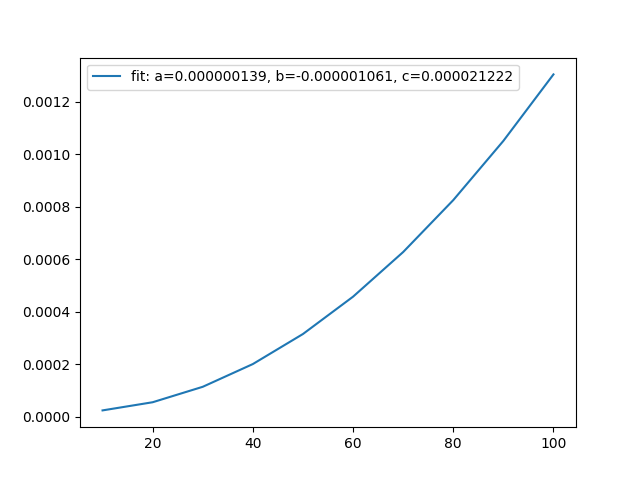
\includegraphics[width=.4\textwidth]{../graficos/seleccion/seleccion.png}
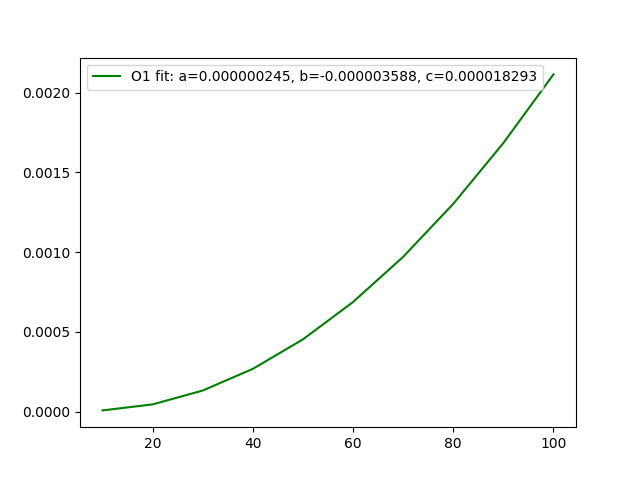
\includegraphics[width=.4\textwidth]{../graficos/seleccion/seleccion_O1.png}
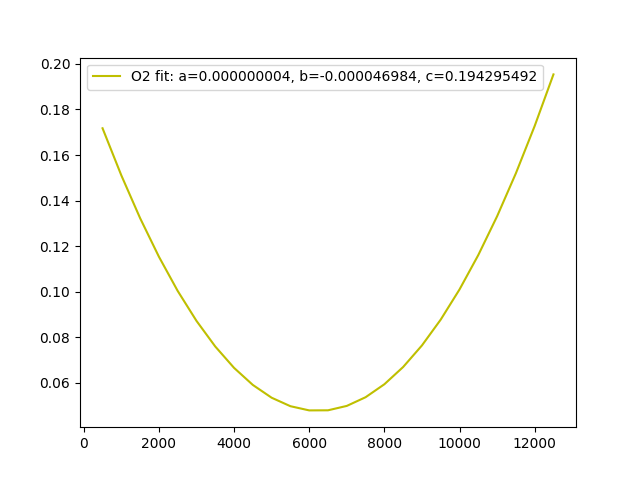
\includegraphics[width=.4\textwidth]{../graficos/seleccion/seleccion_O2.png}
\end{center}
\begin{center}
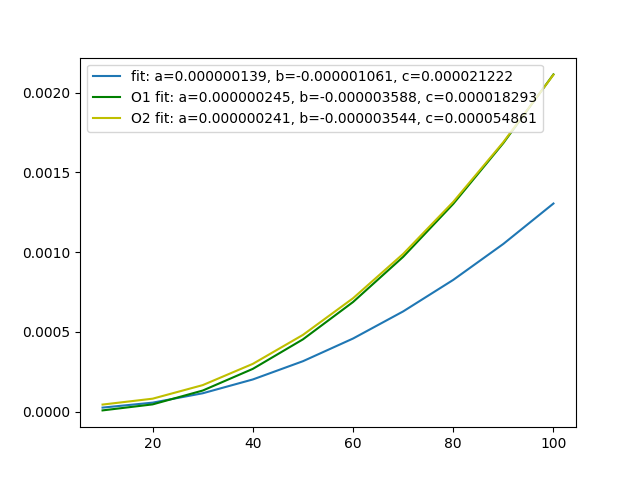
\includegraphics[width=.6\textwidth]{../graficos/seleccion/seleccion_juntas.png}
\end{center}
\begin{center}
\begin{tabular}{| c | c | c | c |}
\hline
\textbf{N} & \textbf{O-} & \textbf{O1} & \textbf{O2} \\ \hline
500 & 0.0314449 & 0.0314842 & 0.0317225 \\ \hline
1000 & 0.119021 & 0.126228 & 0.11633 \\ \hline
1500 & 0.260984 & 0.267642 & 0.258436 \\ \hline
2000 & 0.457069 & 0.461125 & 0.454904 \\ \hline
2500 & 0.00744243 & 0.00693814 & 0.0068266 \\ \hline
3000 & 0.00998253 & 0.0103105 & 0.0104942 \\ \hline
3500 & 0.0138713 & 0.0136245 & 0.0144952 \\ \hline
4000 & 0.0186035 & 0.0182824 & 0.0187636 \\ \hline
4500 & 0.0234744 & 0.0224572 & 0.0237714 \\ \hline
5000 & 0.0277004 & 0.0292558 & 0.0300571 \\ \hline
5500 & 0.0345149 & 0.0354603 & 0.035354 \\ \hline
6000 & 0.0478933 & 0.0406127 & 0.0407739 \\ \hline
6500 & 0.0520387 & 0.0483603 & 0.0474503 \\ \hline
7000 & 0.0560279 & 0.0554717 & 0.0550182 \\ \hline
7500 & 0.0618687 & 0.067223 & 0.0635355 \\ \hline
8000 & 0.0725331 & 0.0711132 & 0.0718062 \\ \hline
8500 & 0.0815797 & 0.0811896 & 0.0813514 \\ \hline
9000 & 0.0909342 & 0.0917913 & 0.0928178 \\ \hline
9500 & 0.103387 & 0.100633 & 0.100902 \\ \hline
10000 & 0.110117 & 0.11207 & 0.127083 \\ \hline
10500 & 0.12314 & 0.124775 & 0.125395 \\ \hline
11000 & 0.134518 & 0.135545 & 0.135101 \\ \hline
11500 & 0.151427 & 0.146785 & 0.146842 \\ \hline
12000 & 0.158935 & 0.163465 & 0.159707 \\ \hline
12500 & 0.174672 & 0.174286 & 0.174868 \\ \hline
\hline
\end{tabular}
\end{center}

\newpage
\subsection{Algoritmo mergesort}
\begin{center}
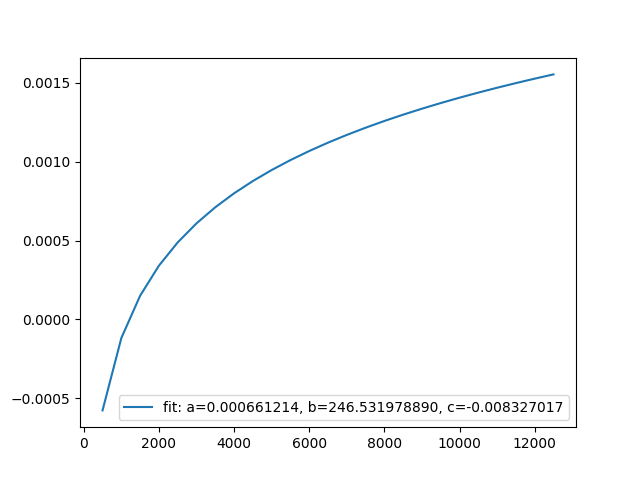
\includegraphics[width=.4\textwidth]{../graficos/mergesort/mergesort.png}
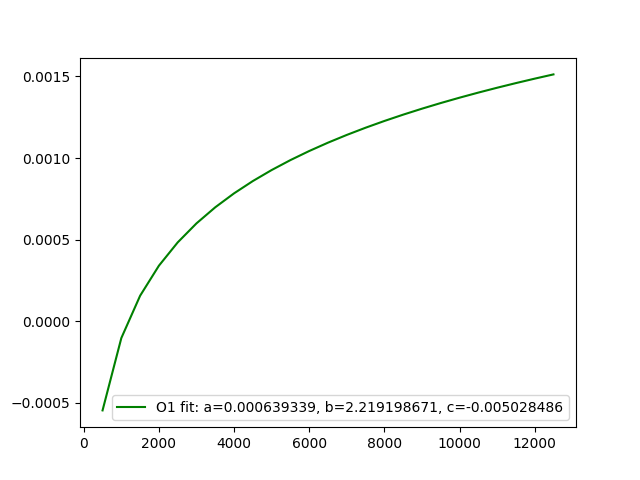
\includegraphics[width=.4\textwidth]{../graficos/mergesort/mergesort_O1.png}
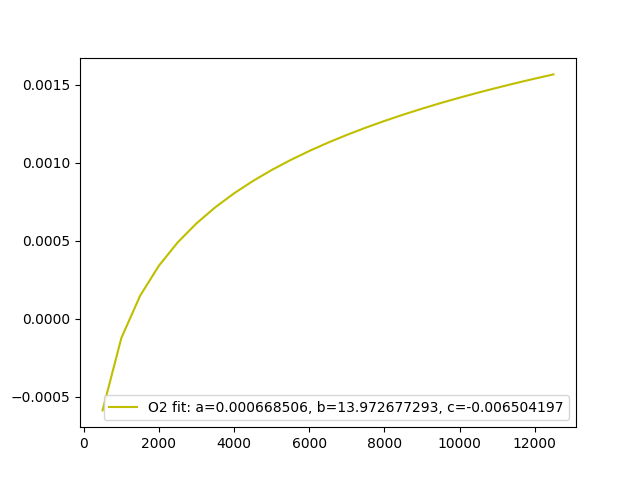
\includegraphics[width=.4\textwidth]{../graficos/mergesort/mergesort_O2.png}
\end{center}
\begin{center}
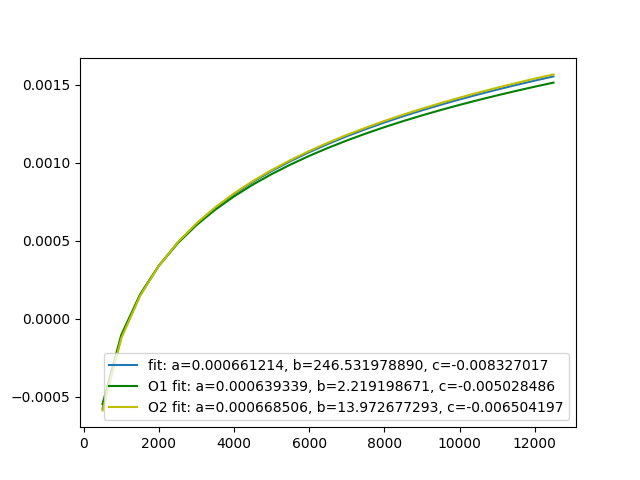
\includegraphics[width=.6\textwidth]{../graficos/mergesort/mergesort_juntas.png}
\end{center}
\begin{center}
\begin{tabular}{| c | c | c | c |}
\hline
\textbf{N} & \textbf{O-} & \textbf{O1} & \textbf{O2} \\ \hline
500 & 4.6913e-05 & 4.2538e-05 & 4.3779e-05 \\ \hline
1000 & 0.000104759 & 0.000101012 & 0.000102685 \\ \hline
1500 & 0.000197928 & 0.000202091 & 0.000197977 \\ \hline
2000 & 0.000230556 & 0.000230267 & 0.000229837 \\ \hline
2500 & 0.000320995 & 0.000321507 & 0.000324846 \\ \hline
3000 & 0.000441303 & 0.000454994 & 0.000459037 \\ \hline
3500 & 0.000411042 & 0.000422831 & 0.000415593 \\ \hline
4000 & 0.000511027 & 0.000494096 & 0.000499695 \\ \hline
4500 & 0.000612995 & 0.000592159 & 0.000609127 \\ \hline
5000 & 0.00069516 & 0.000701389 & 0.000693268 \\ \hline
5500 & 0.000804711 & 0.000800892 & 0.000801765 \\ \hline
6000 & 0.000939736 & 0.0009096 & 0.000922795 \\ \hline
6500 & 0.000810641 & 0.000809706 & 0.000812514 \\ \hline
7000 & 0.000890017 & 0.000891093 & 0.000896917 \\ \hline
7500 & 0.000985485 & 0.000987166 & 0.000983415 \\ \hline
8000 & 0.00110324 & 0.00107382 & 0.00107462 \\ \hline
8500 & 0.00116999 & 0.00116523 & 0.00117428 \\ \hline
9000 & 0.00127648 & 0.00127043 & 0.00127371 \\ \hline
9500 & 0.00138226 & 0.00137334 & 0.00139195 \\ \hline
10000 & 0.00150468 & 0.00148788 & 0.00148267 \\ \hline
10500 & 0.001526 & 0.001525 & 0.001523 \\ \hline
11000 & 0.001634 & 0.001625 & 0.002057 \\ \hline
11500 & 0.001889 & 0.001821 & 0.00186 \\ \hline
12000 & 0.002311 & 0.001866 & 0.002124 \\ \hline
12500 & 0.002148 & 0.002275 & 0.002152 \\ \hline
\hline
\end{tabular}
\end{center}

\newpage
\subsection{Algoritmo quicksort}
\begin{center}
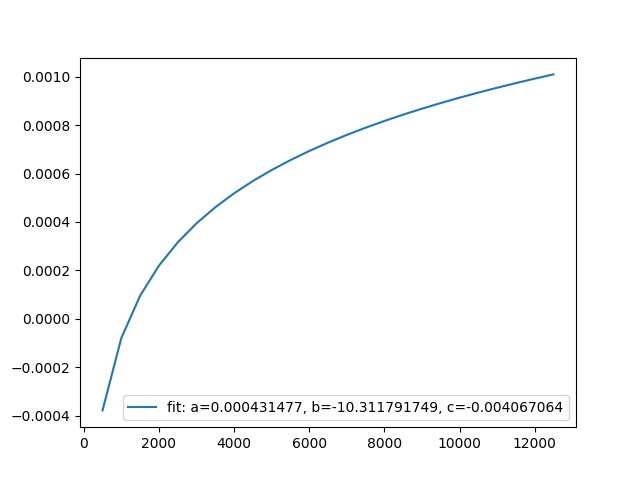
\includegraphics[width=.4\textwidth]{../graficos/quicksort/quicksort.png}
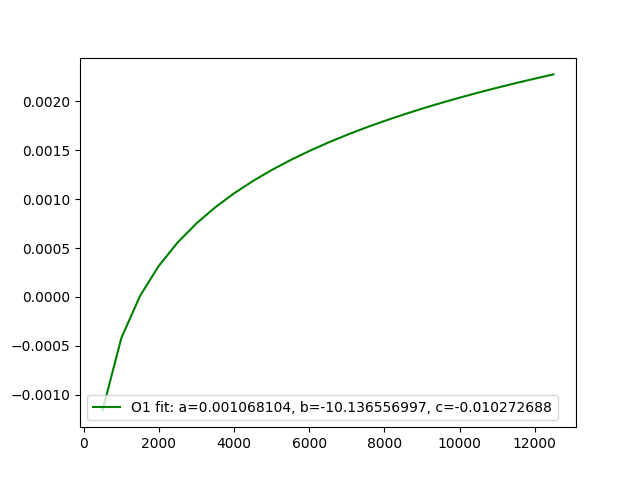
\includegraphics[width=.4\textwidth]{../graficos/quicksort/quicksort_O1.png}
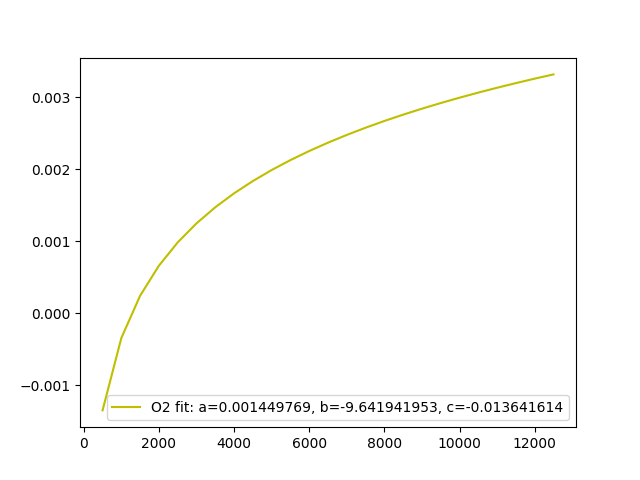
\includegraphics[width=.4\textwidth]{../graficos/quicksort/quicksort_O2.png}
\end{center}
\begin{center}
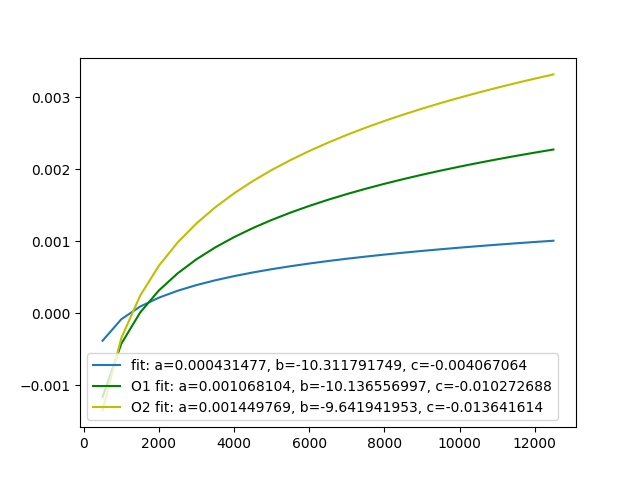
\includegraphics[width=.6\textwidth]{../graficos/quicksort/quicksort_juntas.png}
\end{center}
\begin{center}
\begin{tabular}{| c | c | c | c |}
\hline
\textbf{N} & \textbf{O-} & \textbf{O1} & \textbf{O2} \\ \hline
500 & 3.2332e-05 & 3.7642e-05 & 0.000103603 \\ \hline
1000 & 7.036e-05 & 8.0497e-05 & 0.000222952 \\ \hline
1500 & 0.000113397 & 0.000131637 & 0.000361161 \\ \hline
2000 & 0.000154328 & 0.000176116 & 0.000484841 \\ \hline
2500 & 0.000200578 & 0.00023071 & 0.000631374 \\ \hline
3000 & 0.000240971 & 0.000276572 & 0.000763986 \\ \hline
3500 & 0.000284638 & 0.000360803 & 0.000897255 \\ \hline
4000 & 0.000333301 & 0.000420274 & 0.00107918 \\ \hline
4500 & 0.000373817 & 0.000525212 & 0.001179 \\ \hline
5000 & 0.000419683 & 0.000665588 & 0.00133037 \\ \hline
5500 & 0.000463525 & 0.000837868 & 0.00146456 \\ \hline
6000 & 0.000521563 & 0.000963575 & 0.00166409 \\ \hline
6500 & 0.000557223 & 0.00101092 & 0.0017721 \\ \hline
7000 & 0.000617823 & 0.00132214 & 0.00197305 \\ \hline
7500 & 0.000920243 & 0.00140165 & 0.00211571 \\ \hline
8000 & 0.000714884 & 0.00180813 & 0.00226463 \\ \hline
8500 & 0.000766829 & 0.00193638 & 0.00243405 \\ \hline
9000 & 0.000817047 & 0.00206904 & 0.00260327 \\ \hline
9500 & 0.000909397 & 0.00218516 & 0.00275356 \\ \hline
10000 & 0.000957013 & 0.00232035 & 0.00288264 \\ \hline
10500 & 0.00108144 & 0.00242214 & 0.00302737 \\ \hline
11000 & 0.00115832 & 0.00257706 & 0.00429314 \\ \hline
11500 & 0.00122584 & 0.00265797 & 0.00448855 \\ \hline
12000 & 0.00127122 & 0.00277936 & 0.0046674 \\ \hline
12500 & 0.00135047 & 0.00373325 & 0.00497125 \\ \hline
\hline
\end{tabular}
\end{center}

\newpage
\subsection{Algoritmo heapsort}
\begin{center}
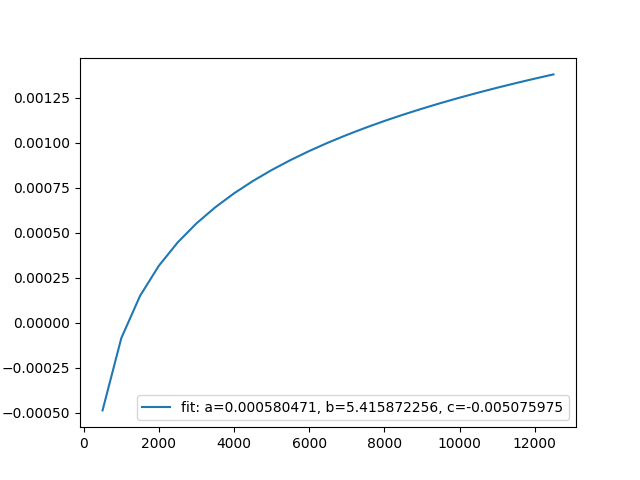
\includegraphics[width=.4\textwidth]{../graficos/heapsort/heapsort.png}
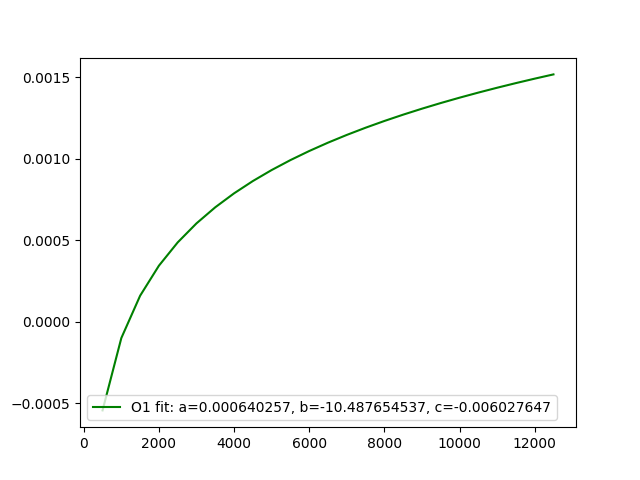
\includegraphics[width=.4\textwidth]{../graficos/heapsort/heapsort_O1.png}
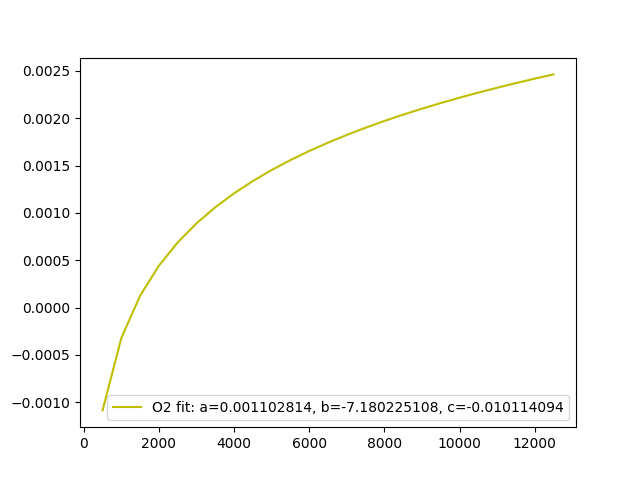
\includegraphics[width=.4\textwidth]{../graficos/heapsort/heapsort_O2.png}
\end{center}
\begin{center}
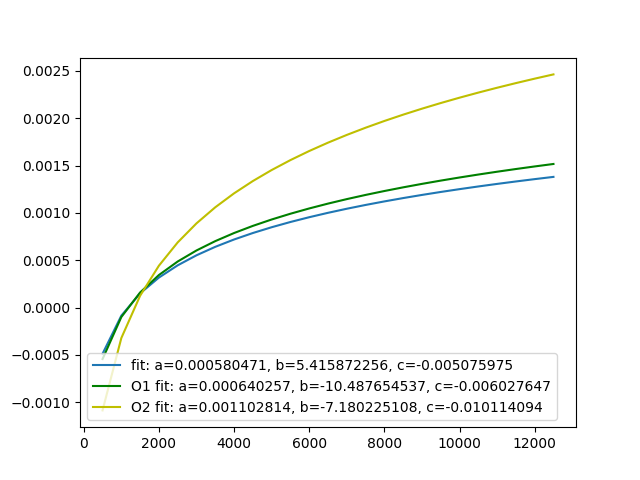
\includegraphics[width=.6\textwidth]{../graficos/heapsort/heapsort_juntas.png}
\end{center}
\begin{center}
\begin{tabular}{| c | c | c | c |}
\hline
\textbf{N} & \textbf{O-} & \textbf{O1} & \textbf{O2} \\ \hline
500 & 4.5886e-05 & 4.7776e-05 & 5.2733e-05 \\ \hline
1000 & 9.3484e-05 & 0.000105841 & 0.000115869 \\ \hline
1500 & 0.000155393 & 0.000165102 & 0.000180243 \\ \hline
2000 & 0.0002156 & 0.000226943 & 0.000250445 \\ \hline
2500 & 0.00027561 & 0.000293035 & 0.000318913 \\ \hline
3000 & 0.000335879 & 0.000370002 & 0.00038954 \\ \hline
3500 & 0.000400699 & 0.000423861 & 0.000472134 \\ \hline
4000 & 0.000462112 & 0.000537971 & 0.00053706 \\ \hline
4500 & 0.000574792 & 0.000613159 & 0.000681049 \\ \hline
5000 & 0.00062758 & 0.000688875 & 0.000936752 \\ \hline
5500 & 0.000696955 & 0.000764817 & 0.00107965 \\ \hline
6000 & 0.000771178 & 0.000843093 & 0.00137774 \\ \hline
6500 & 0.0008542 & 0.000930073 & 0.00153718 \\ \hline
7000 & 0.000948121 & 0.00100329 & 0.0016506 \\ \hline
7500 & 0.000989718 & 0.00108493 & 0.00176835 \\ \hline
8000 & 0.00106711 & 0.00118179 & 0.00193712 \\ \hline
8500 & 0.00113612 & 0.00124409 & 0.00206274 \\ \hline
9000 & 0.00121429 & 0.00132679 & 0.00220556 \\ \hline
9500 & 0.00128797 & 0.00140478 & 0.00231064 \\ \hline
10000 & 0.00136625 & 0.00149198 & 0.00250894 \\ \hline
10500 & 0.00144845 & 0.00157132 & 0.00262056 \\ \hline
11000 & 0.00151039 & 0.00166773 & 0.00271144 \\ \hline
11500 & 0.00158849 & 0.00174876 & 0.00295809 \\ \hline
12000 & 0.00166249 & 0.00188693 & 0.00302842 \\ \hline
12500 & 0.00174171 & 0.00191495 & 0.00311223 \\ \hline
\hline
\end{tabular}
\end{center}

\newpage
\subsection{Algoritmo floyd}
\begin{center}
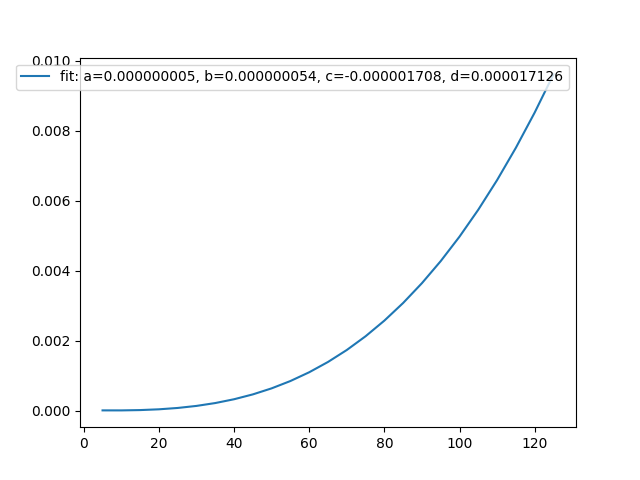
\includegraphics[width=.4\textwidth]{../graficos/floyd/floyd.png}
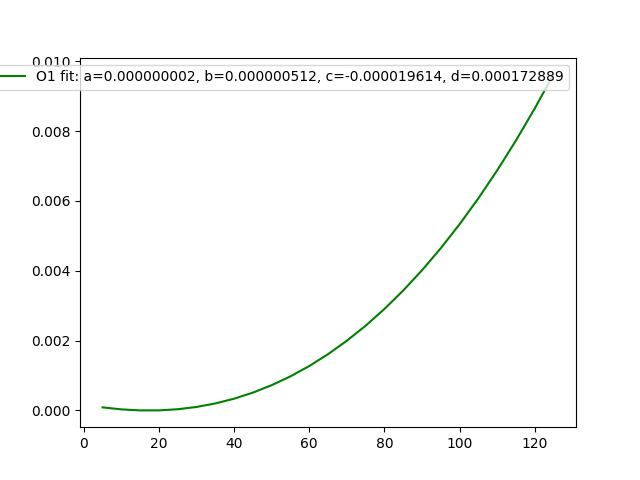
\includegraphics[width=.4\textwidth]{../graficos/floyd/floyd_O1.png}
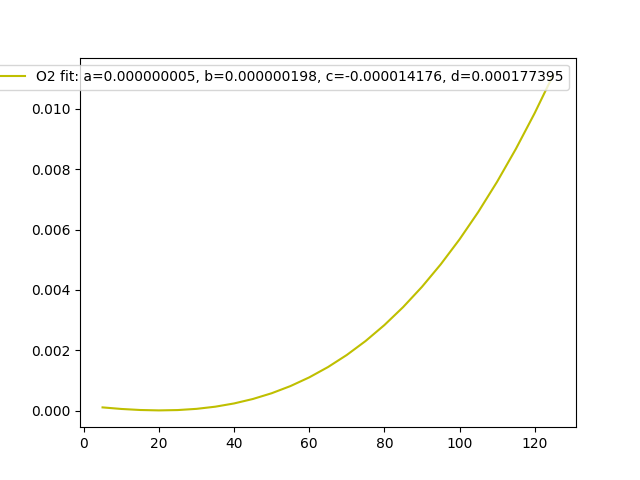
\includegraphics[width=.4\textwidth]{../graficos/floyd/floyd_O2.png}
\end{center}
\begin{center}
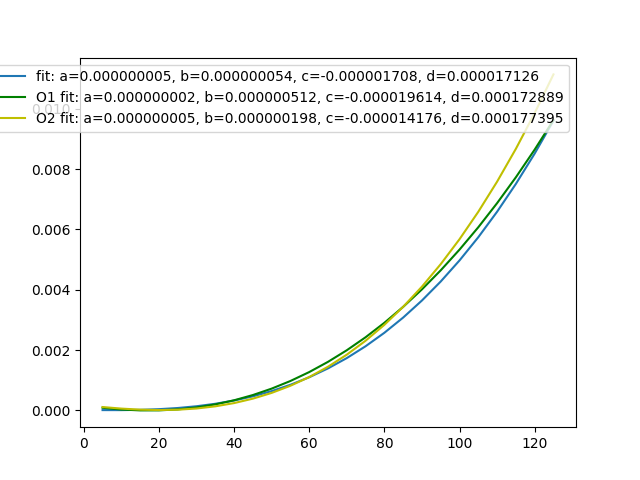
\includegraphics[width=.6\textwidth]{../graficos/floyd/floyd_juntas.png}
\end{center}
\begin{center}
\begin{tabular}{| c | c | c | c |}
\hline
\textbf{N} & \textbf{O-} & \textbf{O1} & \textbf{O2} \\ \hline
5 & 2e-06 & 1e-06 & 2e-06 \\ \hline
10 & 7e-06 & 7e-06 & 7e-06 \\ \hline
15 & 2.1e-05 & 2.1e-05 & 2.1e-05 \\ \hline
20 & 4.6e-05 & 5e-05 & 4.9e-05 \\ \hline
25 & 8.3e-05 & 8.9e-05 & 8.7e-05 \\ \hline
30 & 0.000145 & 0.000149 & 0.000146 \\ \hline
35 & 0.000227 & 0.000244 & 0.00023 \\ \hline
40 & 0.000335 & 0.000377 & 0.000336 \\ \hline
45 & 0.000455 & 0.000512 & 0.000455 \\ \hline
50 & 0.000636 & 0.000731 & 0.000642 \\ \hline
55 & 0.000834 & 0.000952 & 0.000841 \\ \hline
60 & 0.001134 & 0.001233 & 0.001076 \\ \hline
65 & 0.001432 & 0.001545 & 0.001376 \\ \hline
70 & 0.001715 & 0.001924 & 0.001768 \\ \hline
75 & 0.002059 & 0.00235 & 0.002205 \\ \hline
80 & 0.002596 & 0.002852 & 0.002645 \\ \hline
85 & 0.003052 & 0.003377 & 0.003118 \\ \hline
90 & 0.003596 & 0.003975 & 0.004017 \\ \hline
95 & 0.004309 & 0.00473 & 0.004775 \\ \hline
100 & 0.004978 & 0.005552 & 0.005583 \\ \hline
105 & 0.005801 & 0.005681 & 0.006403 \\ \hline
110 & 0.006597 & 0.007624 & 0.009087 \\ \hline
115 & 0.007513 & 0.007536 & 0.008881 \\ \hline
120 & 0.008491 & 0.008468 & 0.009428 \\ \hline
125 & 0.009594 & 0.009587 & 0.010736 \\ \hline
\hline
\end{tabular}
\end{center}

\newpage
\subsection{Algoritmo hanoi}
\begin{center}
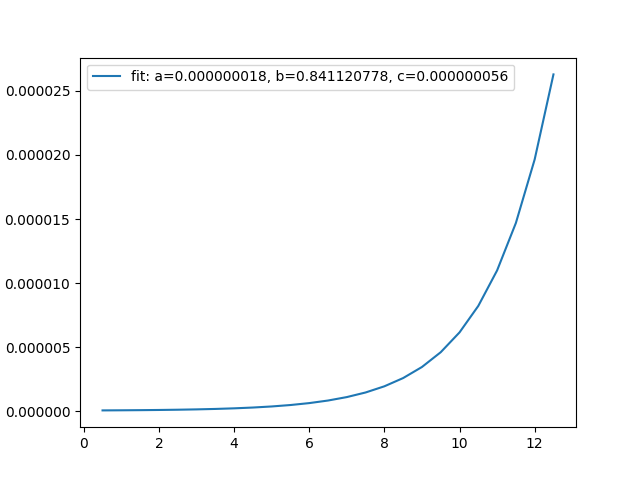
\includegraphics[width=.4\textwidth]{../graficos/hanoi/hanoi.png}
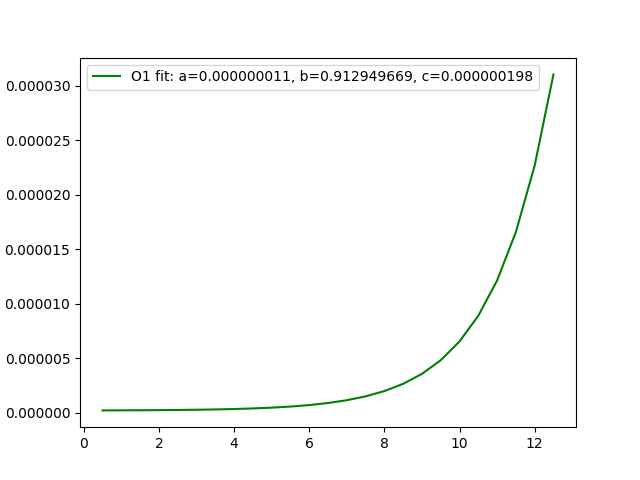
\includegraphics[width=.4\textwidth]{../graficos/hanoi/hanoi_O1.png}
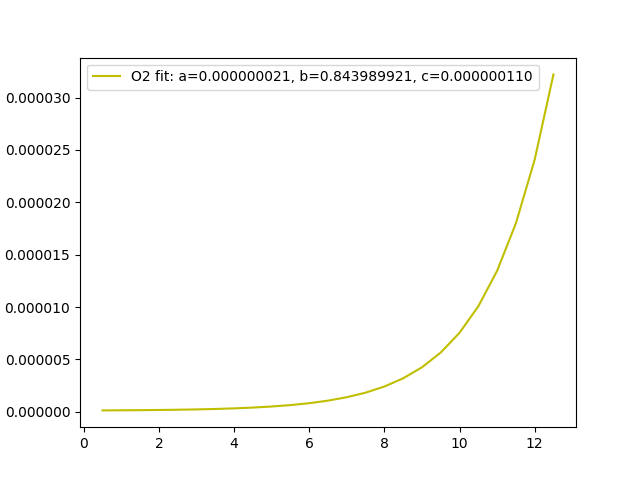
\includegraphics[width=.4\textwidth]{../graficos/hanoi/hanoi_O2.png}
\end{center}
\begin{center}
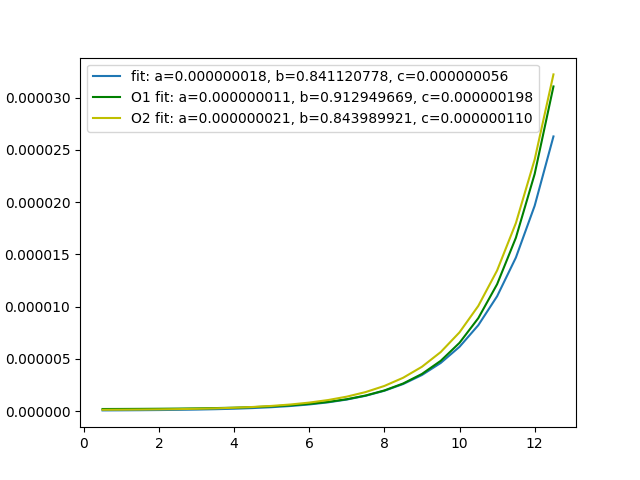
\includegraphics[width=.6\textwidth]{../graficos/hanoi/hanoi_juntas.png}
\end{center}
\begin{center}
\begin{tabular}{| c | c | c | c |}
\hline
\textbf{N} & \textbf{O-} & \textbf{O1} & \textbf{O2} \\ \hline
0.5 & 9.3e-08 & 1.43e-07 & 1.28e-07 \\ \hline
1.0 & 1.71e-07 & 1.6e-07 & 2.97e-07 \\ \hline
1.5 & 1.66e-07 & 1.99e-07 & 1.53e-07 \\ \hline
2.0 & 2.04e-07 & 2.7e-07 & 2.29e-07 \\ \hline
2.5 & 1.41e-07 & 1.45e-07 & 2.08e-07 \\ \hline
3.0 & 2.51e-07 & 2.92e-07 & 3.47e-07 \\ \hline
3.5 & 2.54e-07 & 2.86e-07 & 3.04e-07 \\ \hline
4.0 & 3.91e-07 & 4.69e-07 & 4.54e-07 \\ \hline
4.5 & 3.62e-07 & 4.08e-07 & 4.67e-07 \\ \hline
5.0 & 5.49e-07 & 6.58e-07 & 7.21e-07 \\ \hline
5.5 & 5.26e-07 & 6.2e-07 & 6.98e-07 \\ \hline
6.0 & 8.55e-07 & 9.13e-07 & 1.057e-06 \\ \hline
6.5 & 7.52e-07 & 8.07e-07 & 1.037e-06 \\ \hline
7.0 & 1.16e-06 & 1.374e-06 & 1.563e-06 \\ \hline
7.5 & 1.199e-06 & 1.497e-06 & 1.638e-06 \\ \hline
8.0 & 2.104e-06 & 2.197e-06 & 2.487e-06 \\ \hline
8.5 & 2.187e-06 & 2.384e-06 & 2.744e-06 \\ \hline
9.0 & 3.666e-06 & 3.97e-06 & 4.553e-06 \\ \hline
9.5 & 3.732e-06 & 3.788e-06 & 4.352e-06 \\ \hline
10.0 & 6.565e-06 & 7.148e-06 & 8.174e-06 \\ \hline
10.5 & 6.523e-06 & 7.279e-06 & 8.151e-06 \\ \hline
11.0 & 1.242e-05 & 1.3911e-05 & 1.5101e-05 \\ \hline
11.5 & 1.2321e-05 & 1.365e-05 & 1.5014e-05 \\ \hline
12.0 & 2.4334e-05 & 2.6554e-05 & 2.9694e-05 \\ \hline
12.5 & 2.4104e-05 & 2.9556e-05 & 2.9656e-05 \\ \hline
\hline
\end{tabular}
\end{center}



\section{Algoritmos de búsqueda}
\begin{center}
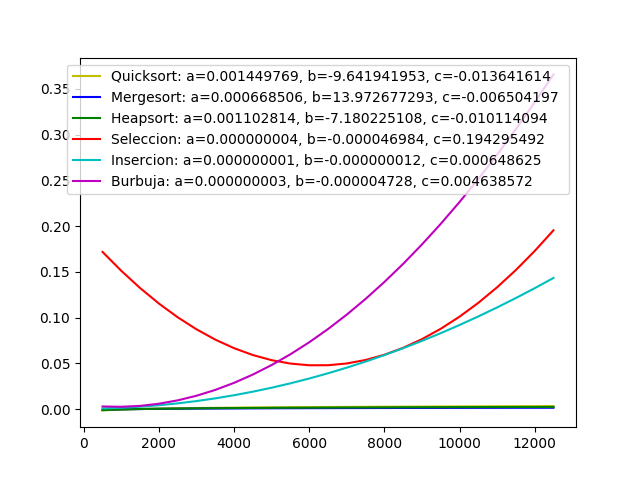
\includegraphics[scale=0.6]{../graficos/ordenacion/ordenacion.png}
\end{center}
En esta gráfica vemos la representación de todos los algoritmos de la práctica, cómo el de burbuja crece mucho más rápidamente que el resto mientras que quicksort, mergesort y heapsort son rectas. Así, concluimos que burbuja > selección > inserción > mergesort, quicksort y heapsort con respecto a eficiencia, algo que veníamos intuyendo al ver que orden tenían al principio del documento.

\begin{center}
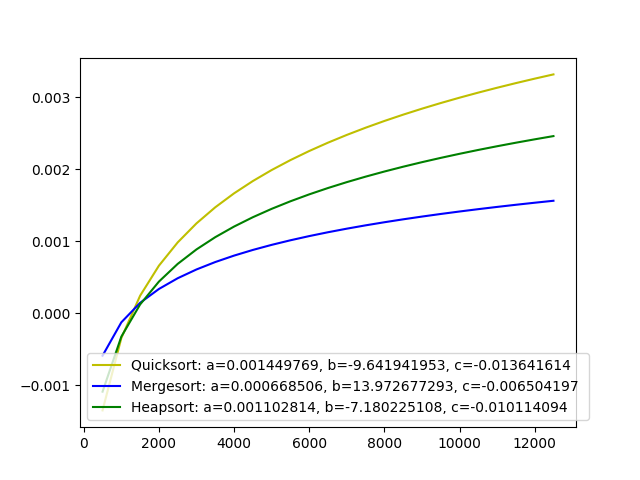
\includegraphics[scale=0.5]{../graficos/ordenacion/ordenacion_sort_only.png}
\end{center}
Para poder diferenciar mejor los algoritmos con O$(n\log(n)$) los vemos en otra gráfica. Apreciamos entonces cómo para tamaños pequeños, hasta 2000 aproximadamente, el algoritmo mergesort es más eficiente que el heapsort, que a su vez es mejor que el quicksort, mas esto cambia y pasa justo lo contrario a partir de 2000.

\end{document}
